\documentclass{article}
\usepackage{graphicx} % Extended graphics inclusions
\usepackage{float}
\usepackage{url} % For \url{}
\usepackage{../config/atxy} % For front cover
\usepackage{amsfonts} % Needed for some fonts
\usepackage[usenames]{color} % Needed for colored R input/output
\usepackage{pdfcolmk} % Correct some problems with the color stack


\title{Nonparametric statistics}
\author{Palmeira, L. \and Lobry, J.R.}

\usepackage{/Library/Frameworks/R.framework/Resources/share/texmf/Sweave}
\begin{document}
%
% To change the R input/output style:
%
\definecolor{Soutput}{rgb}{0,0,0.56}
\definecolor{Sinput}{rgb}{0.56,0,0}
\DefineVerbatimEnvironment{Sinput}{Verbatim}
{formatcom={\color{Sinput}},fontsize=\footnotesize, baselinestretch=0.75}
\DefineVerbatimEnvironment{Soutput}{Verbatim}
{formatcom={\color{Soutput}},fontsize=\footnotesize, baselinestretch=0.75}
%
% This removes the extra spacing after code and output chunks in Sweave,
% but keeps the spacing around the whole block.
%
\fvset{listparameters={\setlength{\topsep}{0pt}}}
\renewenvironment{Schunk}{\vspace{\topsep}}{\vspace{\topsep}}
%
% Rlogo
%
\newcommand{\Rlogo}{\protect
\includegraphics[height=1.8ex,keepaspectratio]{../figs/Rlogo.pdf}}
%
% Shortcut for seqinR:
%
\newcommand{\seqinr}{\texttt{seqin\bf{R}}}
\newcommand{\Seqinr}{\texttt{Seqin\bf{R}}}
\fvset{fontsize= \scriptsize}
%
% R output options and libraries to be loaded.
%
%
%  Sweave Options
%
% Put all figures in the fig folder and start the name with current file name.
% Do not produce EPS files
%


\maketitle
\tableofcontents
% BEGIN - DO NOT REMOVE THIS LINE


\section{Introduction}

Nonparametric statistical methods were initially developped to study
variables for which little or nothing is known concerning their
distribution. This makes them particularly suitable for statistical
analysis of biological sequences, in particular for the study of over-
and under-representation of $k$-letter words (\textit{cf} section 
number \ref{dinu}).

\section{Elementary nonparametric statistics}

\subsection{Introduction}

Those rank statistics are those that were available under the ANALSEQ
software \cite{analseq, acnuc1984}. Formulae were taken from \cite{ChasseJL1988}.
We consider here a sequence
of booleans, for instance:

\begin{Schunk}
\begin{Sinput}
 (x <- rep(c(T, F), 10))
\end{Sinput}
\begin{Soutput}
 [1]  TRUE FALSE  TRUE FALSE  TRUE FALSE  TRUE FALSE  TRUE FALSE  TRUE FALSE
[13]  TRUE FALSE  TRUE FALSE  TRUE FALSE  TRUE FALSE
\end{Soutput}
\end{Schunk}

We note $\mathrm{N}$ the total number of elements in the vector:

\begin{Schunk}
\begin{Sinput}
 (N <- length(x))
\end{Sinput}
\begin{Soutput}
[1] 20
\end{Soutput}
\end{Schunk}

We note $\mathrm{M}$ the total number of TRUE elements in the vector:

\begin{Schunk}
\begin{Sinput}
 (M <- sum(x))
\end{Sinput}
\begin{Soutput}
[1] 10
\end{Soutput}
\end{Schunk}

We note $\omega$ the ranks of TRUE elements:

\begin{Schunk}
\begin{Sinput}
 (omega <- which(x))
\end{Sinput}
\begin{Soutput}
 [1]  1  3  5  7  9 11 13 15 17 19
\end{Soutput}
\end{Schunk}

With one exception, the statistics names are the same as in the ANALSEQ software.

As a practical application, we want to study the isochore structure in \textit{Mus
musculus} chromosome 1 using non-overlapping windows of 100 kb. Data were 
computed this way:

%
% Data saved in *.RData format to avoid long computation
%
\begin{Schunk}
\begin{Sinput}
 choosebank("ensembl")
 n <- 201
 res <- rep(-1, 10 * n)
 chr1 <- paste("MOUSE1_", 1:n, sep = "")
 i <- 1
 for (frag in chr1) {
     myseq <- gfrag(frag, 1, 10^7)
     for (w in seq(1, nchar(myseq), by = 10^5)) {
         res[i] <- GC(s2c(substr(myseq, start = w, stop = w + 
             10^5 - 1)))
         i <- i + 1
     }
 }
 res <- res[res >= 0]
 res[res == 0] <- NA
 res <- 100 * res
 closebank()
 save(res, file = "chr1.RData")
\end{Sinput}
\end{Schunk}

The folowing representation follows the conventions used in Fig 2 from \cite{PacesJ2004}.

\begin{Schunk}
\begin{Sinput}
 load("chr1.RData")
 n <- length(res)
 xx <- seq_len(n)/10
 plot(xx, res, type = "l", las = 1, ylab = "G+C content [%]", 
     main = "Isochores in mouse chromosome 1", xaxt = "n", 
     xlab = "Position on the chromosome [Mb]")
 axis(1, at = seq(0, 200, by = 10))
 breaks <- c(0, 37.5, 42.5, 47.5, 52.5, 100)
 lev <- cut(res, breaks = breaks, labels = c("darkblue", "blue", 
     "yellow", "orange", "red"), ordered = T)
 segments(x0 = xx, y0 = min(res, na.rm = TRUE), x1 = xx, y1 = res, 
     col = as.character(lev), lend = "butt")
 segments(x0 = xx[is.na(res)], y0 = min(res, na.rm = T), x1 = xx[is.na(res)], 
     y1 = max(res, na.rm = T), col = grey(0.7))
 lines(xx, res)
 abline(h = breaks, lty = 3)
\end{Sinput}
\end{Schunk}
\includegraphics[width=1.3\textwidth]{../figs/nonparastats-bernardiplot}

The gray area represent undocumented parts of the chromosome, we won't
consider them in the following and recode the sequence in TRUE and FALSE
if the values are above or below the median, respectively:

\begin{Schunk}
\begin{Sinput}
 yy <- res[!is.na(res)]
 n <- length(yy)
 xx <- seq_len(n)/10
 hline <- median(yy)
 plot(yy ~ xx, type = "n", axes = FALSE, ann = FALSE)
 polygon(c(xx[1], xx, xx[n]), c(min(yy), yy, min(yy)), col = "black", 
     border = NA)
 usr <- par("usr")
 rect(usr[1], usr[3], usr[2], hline, col = "white", border = NA)
 lines(xx, yy)
 abline(h = hline)
 box()
 axis(1)
 axis(2, las = 1)
 title(xlab = "Position on the chromosome [Mb]", ylab = "G+C content [%]", 
     main = "Isochores in mouse chromosome 1")
\end{Sinput}
\end{Schunk}
\includegraphics[width=1.3\textwidth]{../figs/nonparastats-medianplot}

Our logical vector is therefore defined as follows:

\begin{Schunk}
\begin{Sinput}
 appli <- yy > median(yy)
 head(appli)
\end{Sinput}
\begin{Soutput}
[1] FALSE FALSE FALSE FALSE FALSE FALSE
\end{Soutput}
\begin{Sinput}
 tail(appli)
\end{Sinput}
\begin{Soutput}
[1]  TRUE  TRUE FALSE FALSE FALSE  TRUE
\end{Soutput}
\end{Schunk}

\subsection{Rank sum}

The statistic $\mathrm{SR}$ is the sum of the ranks of TRUE elements.

$$
\mathrm{SR} = \sum_{j \in \omega}{j}
$$

\begin{verbatim}
**-***-----------     ==> SR low  (18)
---------***--***     ==> SR high (81)
\end{verbatim}

\begin{eqnarray*}
\mathrm{E(SR)} & = & \mathrm{\frac{M(N + 1)}{2}} \\
\mathrm{V(SR)} & = & \mathrm{\frac{M(N + 1)(N - M)}{12}}
\end{eqnarray*}


\begin{Schunk}
\begin{Sinput}
 SR <- function(bool, N = length(bool), M = sum(bool)) {
     stopifnot(is.logical(bool))
     SR <- sum(seq_len(N)[bool])
     E <- M * (N + 1)/2
     V <- M * (N + 1) * (N - M)/12
     return(list(SR = SR, stat = (SR - E)/sqrt(V)))
 }
 SR(s2c("**-***-----------") == "*")
\end{Sinput}
\begin{Soutput}
$SR
[1] 18

$stat
[1] -2.84605
\end{Soutput}
\begin{Sinput}
 SR(s2c("---------***--***") == "*")
\end{Sinput}
\begin{Soutput}
$SR
[1] 81

$stat
[1] 2.713602
\end{Soutput}
\end{Schunk}

Here is a way to obtain the same result using the standard \Rlogo{} \texttt{wilcox.test()}
function to make a Wilcoxon's rank sum test \cite{WilcoxonF1945}:

\begin{Schunk}
\begin{Sinput}
 SRh <- s2c("---------***--***") == "*"
 x <- seq_len(length(SRh))
 x[!SRh] <- -1 * x[!SRh]
 wilcox.test(x)$statistic
\end{Sinput}
\begin{Soutput}
 V 
81 
\end{Soutput}
\end{Schunk}

The probabilities for all possibe outcomes for the rank sums are given by
\texttt{dwilcox()} but note the $\frac{M(M+1)}{2}$ shift:

\begin{Schunk}
\begin{Sinput}
 m <- sum(SRh)
 n <- length(SRh) - m
 pdf <- dwilcox(x = 0:(n * m), m = m, n = n)
 plot(x = 0:(m * n) + m * (m + 1)/2, y = pdf, xlab = "Possible rank sums", 
     ylab = "Density", main = paste("---------***--*** : N =", 
         length(SRh), "M =", sum(SRh)), pch = 19)
 points(SR(SRh)$SR, dwilcox(x = SR(SRh)$SR - m * (m + 1)/2, 
     m = m, n = n), col = "red", pch = 19)
 arrows(x0 = SR(SRh)$SR, y0 = 0.01, x1 = SR(SRh)$SR, y1 = 0.0015, 
     length = 0.1)
 text(SR(SRh)$SR, 0.01, "Observed\nvalue", pos = 3)
\end{Sinput}
\end{Schunk}
\includegraphics{../figs/nonparastats-demodwilcox}

\noindent\textbf{Real case application}

\begin{Schunk}
\begin{Sinput}
 SR(appli)$stat
\end{Sinput}
\begin{Soutput}
[1] 10.81602
\end{Soutput}
\end{Schunk}

The rank sum is higher than expected at random, there is an excess of GC rich regions
at the rigth end (3'end) of the chromosome.

\subsection{Rank variance}

This statistics is the variance of ranks:

$$
\mathrm{VR} = \sum_{j \in \omega}{(j - \mathrm{\frac{N+1}{2}})^2}
$$

\begin{verbatim}
------****-------    ==> VR low  (6)
***----------****    ==> VR high (323)
\end{verbatim}

\begin{eqnarray*}
\mathrm{E(VR)} & = & \mathrm{\frac{M(N + 1)(N-1)}{12}} \\
\mathrm{V(VR)} & = & \mathrm{\frac{M(N - M)(N + 1)(N + 2)(N - 2)}{180}}
\end{eqnarray*}

\begin{Schunk}
\begin{Sinput}
 VR <- function(bool, N = length(bool), M = sum(bool)) {
     stopifnot(is.logical(bool))
     VR <- sum((seq_len(N)[bool] - (N + 1)/2)^2)
     E <- (M * (N + 1) * (N - 1))/12
     V <- (M * (N - M) * (N + 1) * (N + 2) * (N - 2))/180
     return(list(VR = VR, stat = (VR - E)/sqrt(V)))
 }
 VR(s2c("------****-------") == "*")
\end{Sinput}
\begin{Soutput}
$VR
[1] 6

$stat
[1] -2.337860
\end{Soutput}
\begin{Sinput}
 VR(s2c("***----------****") == "*")
\end{Sinput}
\begin{Soutput}
$VR
[1] 323

$stat
[1] 3.470246
\end{Soutput}
\end{Schunk}

We can use simulations to have an idea of the probability density function
of the rank variance, for instance:

\begin{Schunk}
\begin{Sinput}
 VRh <- s2c("***----------****") == "*"
 simVR <- replicate(5000, VR(sample(VRh))$VR)
 hist(simVR, col = grey(0.7), main = paste("***----------**** : N =", 
     length(VRh), "M =", sum(VRh)), xlab = "Possible rank variances", 
     proba = TRUE)
 lines(density(simVR), lwd = 2)
 arrows(VR(VRh)$VR, 0.004, VR(VRh)$VR, 0, le = 0.1)
\end{Sinput}
\end{Schunk}
\includegraphics{../figs/nonparastats-simVR}

\noindent\textbf{Real case application}

\begin{Schunk}
\begin{Sinput}
 VR(appli)$stat
\end{Sinput}
\begin{Soutput}
[1] 4.587283
\end{Soutput}
\end{Schunk}

The variance of ranks is higher than expected at random, there is an excess of GC rich regions
at the telomeric ends of the chromosome.


\subsection{Clustering around the observed centre}

Let note $\mathrm{C(\omega)}$ the observed centre:

$$
\mathrm{C(\omega)} = \left\{ \begin{array}{rl}
 \omega\left(\mathrm{\frac{M+1}{2}}\right) &\mbox{ if $\mathrm{M}$ is odd} \\
 \omega\left(\mathrm{\frac{M}{2} + 1}\right) &\mbox{ if $\mathrm{M}$ is even}
       \end{array} \right.
$$

The statistic $\mathrm{CC}$\footnote{
the original notation was GC in the ANALSEQ software, we use CC instead to
avoid a collision with the \texttt{GC()} function to compute the G+C content.
} is the dispersion around $\mathrm{C(\omega)}$ is defined by:

$$
\mathrm{CC} = \sum_{j \in \omega}{\left| j - \mathrm{C(\omega)} \right|}
$$

\begin{verbatim}
---*****---------    ==> CC low  (6)
***-------***----    ==> CC high (30)
\end{verbatim}

Noting $\lfloor x \rfloor$ the floor of $x$, we have:

$$
\mathrm{E(CC)} = \mathrm{\frac{(N+1)\lfloor\frac{M}{2}\rfloor\lfloor\frac{M+1}{2}\rfloor}{M+1}}
$$

and

$$
\mathrm{V(CC)} = \left\{ \begin{array}{rl}
 \mathrm{\frac{(M - 1)(M + 3)(N + 1)(N - M)}{48(M + 2)}} &\mbox{ if $\mathrm{M}$ is odd} \\
 \mathrm{\frac{M(N + 1)(N - M)(M^2 + 2*M + 4)}{48(M + 1)^2}} &\mbox{ if $\mathrm{M}$ is even}
       \end{array} \right.
$$

\begin{Schunk}
\begin{Sinput}
 CC <- function(bool, N = length(bool), M = sum(bool)) {
     stopifnot(is.logical(bool))
     C <- median(seq_len(N)[bool])
     GC <- sum(abs(seq_len(N)[bool] - C))
     E <- ((N + 1) * floor(M/2) * floor((M + 1)/2))/(M + 1)
     if (M%%2 == 1) 
         V <- ((M - 1) * (M + 3) * (N + 1) * (N - M))/(48 * 
             (M + 2))
     else V <- (M * (N + 1) * (N - M) * (M^2 + 2 * M + 4))/(48 * 
         (M + 1)^2)
     return(list(GC = GC, stat = (GC - E)/sqrt(V)))
 }
 CC(s2c("---*****---------") == "*")
\end{Sinput}
\begin{Soutput}
$GC
[1] 6

$stat
[1] -2.645751
\end{Soutput}
\begin{Sinput}
 CC(s2c("***-------***----") == "*")
\end{Sinput}
\begin{Soutput}
$GC
[1] 30

$stat
[1] 1.337987
\end{Soutput}
\end{Schunk}

\noindent\textbf{Real case application}

\begin{Schunk}
\begin{Sinput}
 CC(appli)$stat
\end{Sinput}
\begin{Soutput}
[1] 3.266275
\end{Soutput}
\end{Schunk}

The dispersion around the observed centre is higher than expected at random, there is a trend for
GC rich sequences to avoid this centre.



\subsection{Number of runs}

The statistics $\mathrm{NS}$ is the number of runs in the sequence:

\begin{verbatim}
--***---***--***-    ==> NS low  (7)
-*-*-*-*-*-*-*-*-    ==> NS high (17)
\end{verbatim}

\begin{eqnarray*}
\mathrm{E(NS)} & = & \mathrm{\frac{2M(N - M)}{N} + 1} \\
\mathrm{V(NS)} & = & \mathrm{\frac{2M(N - M)(2M(N - M) - N)}{N^2(N - 1)}}
\end{eqnarray*}

\begin{Schunk}
\begin{Sinput}
 NS <- function(bool, N = length(bool), M = sum(bool)) {
     stopifnot(is.logical(bool))
     NS <- length(rle(bool)$lengths)
     DMNmM <- 2 * M * (N - M)
     E <- DMNmM/N + 1
     V <- (DMNmM * (DMNmM - N))/(N * N * (N - 1))
     return(list(NS = NS, stat = (NS - E)/sqrt(V)))
 }
 NS(s2c("--***---***--***-") == "*")
\end{Sinput}
\begin{Soutput}
$NS
[1] 7

$stat
[1] -1.242299
\end{Soutput}
\begin{Sinput}
 NS(s2c("-*-*-*-*-*-*-*-*-") == "*")
\end{Sinput}
\begin{Soutput}
$NS
[1] 17

$stat
[1] 3.786054
\end{Soutput}
\end{Schunk}

The same result can be obtained with the function \texttt{runs.test()} from
package \textbf{tseries} \cite{tseries} this way:

\begin{Schunk}
\begin{Sinput}
 library(tseries)
 NSh <- s2c("-*-*-*-*-*-*-*-*-") == "*"
 tseries::runs.test(as.factor(NSh))$statistic
\end{Sinput}
\begin{Soutput}
Standard Normal 
       3.786054 
\end{Soutput}
\end{Schunk}

\noindent\textbf{Real case application}

\begin{Schunk}
\begin{Sinput}
 NS(appli)$stat
\end{Sinput}
\begin{Soutput}
[1] -33.78859
\end{Soutput}
\end{Schunk}

The number of runs is much less than expected at random, there is a trend for
GC rich sequences to aggregate in consecutive runs: this is the isochore
structure.


\subsection{Multiple clusters}

The statistics $\mathrm{GM}$ is the variance of the length $n_k$ of FALSE runs (including
runs of length zero) between two TRUE. Let note:

\begin{itemize}
\item $n_k(\omega)$ the number of FALSE between $\omega(k-1)$ and $\omega(k)$ for $2 \le k \le \mathrm{M}$.
\item $n_1(\omega)$ the number of FALSE before $\omega(1)$.
\item $n_{\mathrm{M+1}}(\omega)$ the number of FALSE after $\omega(\mathrm{M})$.
\end{itemize}

$$
\mathrm{GM} = \frac{1}{\mathrm{M}}\sum_{i = 1}^{\mathrm{M+1}}{\left( n_i(\omega) - \mathrm{\frac{N-M}{M+1}} \right)^2}
$$

\begin{verbatim}
-*-*-*-*-*-*-*-*-    ==> GM low  (0)
***------***-***-    ==> GM high (3.5)
\end{verbatim}

\begin{eqnarray*}
\mathrm{E(GM)} & = & \mathrm{\frac{(N + 1)(N - M)}{(M +1)(M + 2)}} \\
\mathrm{V(GM)} & = & \mathrm{\frac{4(N - M - 1)(N + 1)(N + 2)(N - M)}{M(M + 2)^2(M + 3)(M + 4)}}
\end{eqnarray*}

\begin{Schunk}
\begin{Sinput}
 GM <- function(bool, N = length(bool), M = sum(bool)) {
     stopifnot(is.logical(bool))
     XGM <- (N - M)/(M + 1)
     LS0 <- GM <- 0
     for (i in seq_len(N)) {
         if (bool[i]) {
             GM <- GM + (LS0 - XGM)^2
             LS0 <- 0
         }
         else {
             LS0 <- LS0 + 1
         }
     }
     GM <- (GM + (LS0 - XGM)^2)/M
     E <- ((N + 1) * (N - M))/((M + 1) * (M + 2))
     V <- (4 * (N - M - 1) * (N + 1) * (N + 2) * (N - M))/(M * 
         (M + 2)^2 * (M + 3) * (M + 4))
     return(list(GM = GM, stat = (GM - E)/sqrt(V)))
 }
 GM(s2c("-*-*-*-*-*-*-*-*-") == "*")
\end{Sinput}
\begin{Soutput}
$GM
[1] 0

$stat
[1] -1.863782
\end{Soutput}
\begin{Sinput}
 GM(s2c("***------***-***-") == "*")
\end{Sinput}
\begin{Soutput}
$GM
[1] 3.511111

$stat
[1] 3.279144
\end{Soutput}
\end{Schunk}

\noindent\textbf{Real case application}

\begin{Schunk}
\begin{Sinput}
 GM(appli)$stat
\end{Sinput}
\begin{Soutput}
[1] 320.8337
\end{Soutput}
\end{Schunk}

The number of cluster is much higher than expected at random, there is a trend for
GC rich sequences to aggregate in clusters: this is again the reflect of the isochore
structure in this chromosome.

\section{Dinucleotides over- and under-representation}
\label{dinu}

\subsection{Introduction}

We will briefly describe two statistics for the measure of
dinucleotide over- and under-representation in sequences
\cite{Karlin,UV}, which can both be computed with \seqinr{}. We will
subsequently use them to answer the long-time controversial question
concerning the relationship between UV exposure and genomic content in
bacteria \cite{Singer,Bak}.

\subsection{The \textit{rho} statistic}

The $\rho$ statistic (\texttt{rho()}), presented in \cite{Karlin},
measures the over- and under-representation of two-letter words:

$$\rho(xy) = \frac{f_{xy}}{f_{x}\times f_{y}}$$

where $f_{xy}$ and $f_{x}$ are respectively the frequencies of
dinucleotide $xy$ and nucleotide $x$ in the studied sequence. The
underlying model of random generation considers dinucleotides to be
formed according to the specific frequencies of the two nucleotides
that compose it ($\rho_{xy} = 1$). Departure from this value
characterizes either over- or under-representation of dinucleotide
$xy$.


We expect the $\rho$ statistic of a randomly generated sequence to be
neither over- nor under-represented. Indeed, when we compute the
$\rho$ statistic on 500 random
sequences, we can fit a normal distribution which is centered on 1
(see Fig. \ref{rho})

\begin{Schunk}
\begin{Sinput}
 set.seed(1)
 n <- 500
 di <- 4
 lseq <- 6000
 rhoseq <- replicate(n, rho(sample(s2c("acgt"), size = lseq, 
     replace = TRUE)))
 x <- seq(min(rhoseq[di, ]), max(rhoseq[di, ]), length.out = 1000)
 y <- dnorm(x, mean = mean(rhoseq[di, ]), sd = sd(rhoseq[di, 
     ]))
 histo <- hist(rhoseq[di, ], plot = FALSE)
 plot(histo, freq = FALSE, xlab = expression(paste(rho, " statistic")), 
     main = paste("Distribution for dinucleotide", toupper(labels(rhoseq)[[1]][di]), 
         "on", n, "random sequences"), las = 1, col = grey(0.8), 
     border = grey(0.5), ylim = c(0, max(c(y, histo$density))))
 lines(x, y, lty = 1, col = "red")
 abline(v = 1, lty = 3, col = "blue", lwd = 2)
 legend("topleft", inset = 0.01, legend = c("normal fit", expression(paste(rho, 
     " = 1"))), lty = c(1, 3), col = c("red", "blue"), lwd = c(1, 
     2))
\end{Sinput}
\end{Schunk}

\begin{figure}
\centering\fbox{
\begin{minipage}{\textwidth}
\centering
\includegraphics[width=\textwidth]{../figs/nonparastats-rho}
\caption{Distribution of the $\rho$ statistic computed on
     500 random sequences of
      length 6000. The vertical
     dotted line is centered on 1. The curve draws the fitted normal
     distribution.}
\label{rho}
\end{minipage}
}
\end{figure}

The downside of this statistic, is that the model against which we
compare the sequence under study is fixed. For several types of
sequences, dinucleotides are far from being formed by mere chance
(CDS, ...). In this case, the model used in the $\rho$ statistic
becomes trivial, and the over- or under-representations measured are
mainly due to the strong constraints acting on those sequences.

\subsection{The $z$-score statistic}

The $z$-score statistic (\texttt{zscore()}) is inspired by the
$\rho$ statistic, and is defined so that several different models can
be used for the determination of over- and under-representation
\cite{UV}. It allows for a finer measure of over- and
under-representation in sequences, according to the chosen model.

The $z$-score is defined as follows:

$$z_{score}=\frac{\rho_{xy}-E(\rho_{xy})}{\sqrt{Var(\rho_{xy})}}$$

where $E(\rho_{xy})$ and $Var(\rho_{xy})$ are the expected mean and
variance of $\rho_{xy}$ according to a given model that describes the
sequence.

This statistic follows the standard normal distribution, and can be
computed with several different models of random sequence generation
based on permutations from the original sequence (\texttt{modele}
argument). More details on those models can be obtained in the
documentation for the \texttt{zscore()} function, by simply typing
\texttt{?zscore}.

For instance, if we want to measure the over- and under-representation
of dinucleotides in CDS sequences, we can use the \texttt{codon}
model, which measures the over- and under-representations existing in
the studied sequence once codon usage bias has been erased. For
intergenic sequences, or sequences for which no good permutation model
can be established, we can use the \texttt{base} model. 

\subsection{Comparing statistics on a sequence}

Let's have a look at what these different statistics can show. First,
we will extract a CDS sequence of \textit{Escherichia coli}'s
chromosome from the Genome Reviews database. Let's use, for instance, 
the following CDS:

\begin{Schunk}
\begin{Sinput}
 choosebank("greview")
 query("coli", "N=U00096 ET T=CDS ET K=2.3.1.79@")
 sequence <- getSequence(coli$req[[1]])
 annot <- getAnnot(coli$req[[1]])
 closebank()
 cat(annot, sep = "\n")
\end{Sinput}
\begin{Soutput}
FT   CDS             complement(478591..479142)
FT                   /codon_start=1
FT                   /gene="maa {UniProt/Swiss-Prot:P77791}"
FT                   /locus_tag="b0459 {UniProt/Swiss-Prot:P77791}"
FT                   /product="Maltose O-acetyltransferase
FT                   {UniProt/Swiss-Prot:P77791}"
FT                   /EC_number="2.3.1.79 {UniProt/Swiss-Prot:P77791}"
FT                   /function="maltose O-acetyltransferase activity
FT                   {GO:0008925}"
FT                   /protein_id="AAC73561.1 {EMBL:U00096}"
FT                   /db_xref="EMBL:AAB40214.1 {UniProt/Swiss-Prot:P77791}"
FT                   /db_xref="EMBL:CAA11147.1 {UniProt/Swiss-Prot:P77791}"
FT                   /db_xref="EcoGene:EG14239 {UniProt/Swiss-Prot:P77791}"
FT                   /db_xref="GO:0008925 {GOA:P77791}"
FT                   /db_xref="HOGENOM:HBG023156 {HogenProt:P77791}"
FT                   /db_xref="InterPro:IPR001451 {UniProt/Swiss-Prot:P77791}"
FT                   /db_xref="InterPro:IPR011004 {UniProt/Swiss-Prot:P77791}"
FT                   /db_xref="UniParc:UPI000002EA96 {EMBL:AAC73561}"
FT                   /db_xref="UniProt/Swiss-Prot:P77791 {EMBL:U00096}"
FT                   /transl_table=11
FT                   /translation="MSTEKEKMIAGELYRSADETLSRDRLRARQLIHRYNHSLAEEHTL
FT                   RQQILADLFGQVTEAYIEPTFRCDYGYNIFLGNNFFANFDCVMLDVCPIRIGDNCMLAP
FT                   GVHIYTATHPIDPVARNSGAELGKPVTIGNNVWIGGRAVINPGVTIGDNVVVASGAVVT
FT                   KDVPDNVVVGGNPARIIKKL"
FT                   /%(C+G)="CG<50%"
FT                   /note="C+G content in third codon positions = 47.8 % "
\end{Soutput}
\end{Schunk}

We can see
that this CDS encodes a maltose O-acetyltransferase protein. 
We will now compare the three
following nonparametric statistics:

\begin{itemize}
\item the $\rho$ statistic,
\item the $z$-score statistic with \texttt{base} model,
\item and the $z$-score statistic with \texttt{codon} model.
\end{itemize}

The $z$-score statistic has been modified to incorporate an exact
analytical calculation of the \texttt{base} model where the old 
version (seqinR 1.1-1 and previous versions) incorporated an
approximation for large sequences. This has been possible with the
help of Sophie Schbath \cite{Schbath-thesis}, and the new version of
this calculation can be obtained with the argument \texttt{exact} 
set to \texttt{TRUE} (\texttt{FALSE} being the default). 
The analytical solution for the \texttt{codon} model is from \cite{GautierC1985}.
The following
code was used to produce figure \ref{dinuclcoli}:

\begin{Schunk}
\begin{Sinput}
 rhocoli <- rho(sequence)
 zcolibase <- zscore(sequence, model = "base", exact = TRUE)
 zcolicodon <- zscore(sequence, model = "codon", exact = TRUE)
 par(mfrow = c(3, 1), lend = "butt", oma = c(0, 0, 2, 0), mar = c(3, 
     4, 0, 2))
 col <- c("green", "blue", "orange", "red")
 plot(rhocoli - 1, ylim = c(-0.5, 0.5), las = 1, ylab = expression(rho), 
     lwd = 10, xaxt = "n", col = col)
 axis(1, at = 1:16, labels = toupper(words(2)))
 abline(h = 0)
 plot(zcolibase, ylim = c(-2.5, 2.5), las = 1, ylab = "zscore with base model", 
     lwd = 10, xaxt = "n", col = col)
 axis(1, at = 1:16, labels = toupper(words(2)))
 abline(h = 0)
 plot(zcolicodon, ylim = c(-2.5, 2.5), las = 1, ylab = "zscore with codon model", 
     lwd = 10, xaxt = "n", col = col)
 axis(1, at = 1:16, labels = toupper(words(2)))
 abline(h = 0)
 mtext("Comparison of the three statistics", outer = TRUE, 
     cex = 1.5)
\end{Sinput}
\end{Schunk}

\begin{figure}
\centering\fbox{
\begin{minipage}{\textwidth}
\centering
\includegraphics[width=\textwidth]{../figs/nonparastats-dinuclcoli}
   \caption{Three different non-parametric statistics (from left to
   right: $\rho$, $zscore$ with \texttt{base} model, $zscore$ with
   \texttt{codon} model), computed on the same sequence from
   \textit{Escherichia coli}. In order to make the figures easily
   comparable, we substracted 1 to the \texttt{rho()} results, so that
   all 3 statistics are centered at 0. }
\label{dinuclcoli}
\end{minipage}
}
\end{figure}

The first two panels in figure \ref{dinuclcoli} are almost identical: 
this is due to the way the
$z$-score statistic has been built. The statistic computed with
the \texttt{base} model is a reflection of the $\rho$ statistic. The
difference being that the $z$-score follows a standard normal
distribution, which makes easier the comparisons between the results
from the \texttt{base} model and the ones from the \texttt{codon}
model. The last pannel ($z$-score with \texttt{codon} model), is
completely different: almost all over- and under-representations have
been erased. We can safely say that these over- and
under-representations were due to codon usage bias.

On the last panel, four dinucleotides stand out: CC and TT seem
rather under-represented, CT and TC rather over-represented. This
means that, in this sequence, codons ending with a given pyrimidine
tend to be more frequently followed by a codon starting with the other
pyrimidine than expected by chance. This is not a universal feature of
\textit{Escherichia coli}, and is probably due to the amino-acid
composition of this particular sequence. It seemed a funny example, as
the following part will also relate to pyrimidine dinucleotides.
However, what we see on this CDS from \textit{Escherichia coli} has
nothing to do with what follows...

\section{UV exposure and dinucleotide content}

In the beginning of the 1970's, two contradictory papers considered
the question of the impact of UV exposure on genomic content. Both
papers had strong arguments for either side, and the question remained
open until recently \cite{UV}.

\subsection{The expected impact of UV light on genomic content}

On this controversy, the known facts are: pyrimidine dinucleotides
(CC, TT, CT and TC) are the major DNA target for UV-light
\cite{Setlow}; the sensitivities of the four pyrimidine dinucleotides
to UV wavelengths differ and depend on the micro-organism
\cite{Setlow}:

\begin{table}[H]
\begin{center}
\begin{tabular}{rcccc}
  \hline \hline
  & G+C content & CC (\%) & CT + TC (\%) & TT (\%)\\
  \hline
  \textit{Haemophilus influenzae} & 62 & 5 & 24 & 71 \\
  \textit{Escherichia coli} & 50 & 7 & 34 & 59 \\
  \textit{Micrococcus lysodeikticus} & 30 & 26 & 55 & 19 \\
  \hline \hline
\end{tabular}
\caption{Proportion of dimers formed in the DNA of three bacteria
  after irradiation with 265 nm UV light. Table adapted from
  \cite{Setlow}.}
\label{sensitivity}
\end{center}
\end{table}



The hypothesis presented by Singer and Ames \cite{Singer} is that
pyrimidine dinucleotides are avoided in light-exposed micro-organisms.
At the time, only G+C content is available, and -- based exclusively
on the sensitivity of the four pyrimidine dinucleotides in an
\textit{Escherichia coli} chromosome -- they hypothesize that a high
G+C will result in less pyrimidine target. Indeed, they find that
bacteria exposed to high levels of UV have higher G+C content than the
others. Bak \textit{et al.} \cite{Bak} strongly criticize their
methodology, but no clear cut answer is achieved.

In an \textit{Escherichia coli} chromosome, it is true that a sequence
with a high G+C content will contain few phototargets: the following
code was used to produce figure \ref{GCcoli}.

\begin{Schunk}
\begin{Sinput}
 worstcase <- function(gc) {
     c <- gc
     t <- (1 - gc)
     (0.59 * t * t + 0.34 * t * c + 0.07 * c * c)/2
 }
 randomcase <- function(gc) {
     c <- gc/2
     t <- (1 - gc)/2
     0.59 * t * t + 0.34 * t * c + 0.07 * c * c
 }
 bestcase <- function(gc) {
     c <- (gc)/2
     t <- (1 - gc)/2
     if ((c + t) <= 0.5) {
         0
     }
     else {
         c <- (c + t - 0.5)/2
         t <- (c + t - 0.5)/2
         0.59 * t * t + 0.34 * t * c + 0.07 * c * c
     }
 }
 xval <- seq(from = 0, to = 100, length = 100)
 yrand <- sapply(xval/100, randomcase)
 yworst <- sapply(xval/100, worstcase)
 ybest <- sapply(xval/100, bestcase)
 plot(xval, 100 * yworst, las = 1, type = "l", lwd = 2, lty = 1, 
     xlab = "G+C content [%]", ylab = "Phototargets weighted density [%]", 
     main = "Estimated as in Escherichia coli chromosome", 
     ylim = c(0, max(100 * yworst)))
 points(xval, 100 * yrand, type = "l", lwd = 2, lty = 2)
 points(xval, 100 * ybest, type = "l", lwd = 2, lty = 3)
 abline(v = c(25, 75), lty = 2)
 arrows(25, 25, 75, 25, code = 1, le = 0.1)
 arrows(25, 25, 75, 25, code = 2, le = 0.1)
 text(50, 25, "Biological range", pos = 3)
\end{Sinput}
\end{Schunk}

\begin{figure}
\centering\fbox{
\begin{minipage}{\textwidth}
\centering
\includegraphics[width=\textwidth]{../figs/nonparastats-GCcoli}
\caption{Density of phototargets, weighted by their frequency in the
  \textit{Escherichia coli} chromosome, and calculated for different
  G+C contents and for three kinds of random genomes. The weights are
  as follows: $0.59*f_{tt}+0.34*(f_{tc}+f_{ct})+0.07*f_{cc}$ (where
  $f_{xy}$ is the frequency of dinucleotide $xy$ in the specified
  genome). Three models of random genomes are analyzed. In the worst
  case (solid curve), the genome is the concatenation of a sequence of
  pyrimidines and a sequence of purines: all pyrimidines are involved
  in a pyrimidine dinucleotide. In the best case (dotted curve), the
  genome is an unbroken succession of pyrimidine-purine dinucleotides:
  no pyrimidine is involved in a pyrimidine dinucleotide. In the
  "random case" (dashed curve), the frequency of a pyrimidine
  dinucleotide is the result of chance ($f_{xy} = f_{x}\times
  f_{y}$).}
\label{GCcoli}
\end{minipage}
}
\end{figure}


In a \textit{Micrococcus lysodeikticus} sequence (the following code
was used to produce figure \ref{GCmicro}), we can see that this 
is no longer true...

\begin{Schunk}
\begin{Sinput}
 worstcase <- function(gc) {
     c <- gc
     t <- (1 - gc)
     (0.19 * t * t + 0.55 * t * c + 0.26 * c * c)/2
 }
 randomcase <- function(gc) {
     c <- gc/2
     t <- (1 - gc)/2
     0.19 * t * t + 0.55 * t * c + 0.26 * c * c
 }
 bestcase <- function(gc) {
     c <- (gc)/2
     t <- (1 - gc)/2
     if ((c + t) <= 0.5) {
         0
     }
     else {
         c <- (c + t - 0.5)/2
         t <- (c + t - 0.5)/2
         0.19 * t * t + 0.55 * t * c + 0.26 * c * c
     }
 }
 xval <- seq(from = 0, to = 100, length = 100)
 yrand <- sapply(xval/100, randomcase)
 yworst <- sapply(xval/100, worstcase)
 ybest <- sapply(xval/100, bestcase)
 plot(xval, 100 * yworst, las = 1, type = "l", lwd = 2, lty = 1, 
     xlab = "G+C content [%]", ylab = "Phototargets weighted density [%]", 
     main = "Estimated as in Micrococcus lysodeikticus chromosome", 
     ylim = c(0, max(100 * yworst)))
 points(xval, 100 * yrand, type = "l", lwd = 2, lty = 2)
 points(xval, 100 * ybest, type = "l", lwd = 2, lty = 3)
 abline(v = c(25, 75), lty = 2)
 arrows(25, 25, 75, 25, code = 1, le = 0.1)
 arrows(25, 25, 75, 25, code = 2, le = 0.1)
 text(50, 25, "Biological range", pos = 3)
\end{Sinput}
\end{Schunk}

\begin{figure}
\centering\fbox{
\begin{minipage}{\textwidth}
\centering
\includegraphics[width=\textwidth]{../figs/nonparastats-GCmicro}
\caption{Density of phototargets, weighted by their frequency in the
  \textit{Micrococcus lysodeikticus} chromosome, and calculated for
  different G+C contents and for three kinds of random genomes. The
  weights are as follows:
  $0.19*f_{tt}+0.55*(f_{tc}+f_{ct})+0.26*f_{cc}$. See figure \ref{GCcoli}
  for more details.}
\label{GCmicro}
\end{minipage}
}
\end{figure}

These two figures (figure \ref{GCcoli} and \ref{GCmicro}) show 
that the density of phototargets depends on:

\begin{itemize}
\item the degree of aggregation of pyrimidine dinucleotides in the
sequence,
\item the sensitivities of the four pyrimidine dinucleotides.
  \end{itemize}

Instead of looking at G+C content, which is an indirect measure of the
impact of UV exposure on genomic content, let us look at pyrimidine
dinucleotide content.

Are CC, TT, CT and TC dinucleotides avoided in light-exposed bacteria?

\subsection{The measured impact of UV light on genomic content}

On all available genomes (as retrieved from Genome Reviews database on
June 16, 2005), we have computed the mean of the $z$-score with
the \texttt{base} model on all intergenic sequences, and the mean of
the $z$-score with the \texttt{codon} model on all CDS.
The results show that there is no systematic under-representation of
none of the four pyrimidine dinucleotides (see figure
\ref{dinucl-graphes} produced by the following code).

\begin{Schunk}
\begin{Sinput}
 data(dinucl)
 par(mfrow = c(2, 2), mar = c(4, 4, 0.5, 0.5) + 0.1)
 myplot <- function(x) {
     plot(dinucl$intergenic[, x], dinucl$coding[, x], xlab = "intergenic", 
         ylab = "coding", las = 1, ylim = c(-6, 4), xlim = c(-3, 
             3), cex = 0)
     rect(-10, -10, -1.96, 10, col = "yellow", border = "yellow")
     rect(1.96, -10, 10, 10, col = "yellow", border = "yellow")
     rect(-10, -10, 10, -1.96, col = "yellow", border = "yellow")
     rect(-10, 1.96, 10, 10, col = "yellow", border = "yellow")
     abline(v = 0, lty = 3)
     abline(h = 0, lty = 3)
     abline(h = -1.96, lty = 2)
     abline(h = +1.96, lty = 2)
     abline(v = -1.96, lty = 2)
     abline(v = +1.96, lty = 2)
     points(dinucl$intergenic[, x], dinucl$coding[, x], pch = 21, 
         col = rgb(0.1, 0.1, 0.1, 0.5), bg = rgb(0.5, 0.5, 
             0.5, 0.5))
     legend("bottomright", inset = 0.02, legend = paste(substr(x, 
         1, 1), "p", substr(x, 2, 2), " bias", sep = ""), cex = 1.25, 
         bg = "white")
     box()
 }
 myplot("CT")
 myplot("TC")
 myplot("CC")
 myplot("TT")
\end{Sinput}
\end{Schunk}

\begin{figure}
\centering\fbox{
\begin{minipage}{\textwidth}
\centering
\includegraphics[width=\textwidth]{../figs/nonparastats-dinucl-graphes}
   \caption{Plot of the mean $zscore$ statistics for
   \textbf{intergenic sequences} (x-axis) and for \textbf{coding
   sequences} (y-axis), for each of the four pyrimidine dinucleotides.
   On each plot, a dot corresponds to the mean of these two statistics
   in a given prokaryote chromosome. The null x and y axis (dotted
   lines), and the 5\% limits of significance for the standard normal
   distribution (dashed lines) are plotted as benchmarks. It should be
   noted that the variability within one chromosome is sometimes as
   great as that between different chromosomes.}
\label{dinucl-graphes}
\end{minipage}
}\end{figure}

However, we have little or no information on the exposure of this
bacteria to UV light. In order to fully answer this question, let's do
another analysis and look at \textit{Prochlorococcus marinus} genome.

\textit{Prochlorococcus marinus} seems to make an ideal model for
investigating this hypothesis. Three completely sequenced strains are
available in the Genome reviews database: two of these strains are
adpated to living at a depth of more than 120 meters (accession
numbers AE017126 and BX548175), and the other one at a depth of 5
meters (accession number BX548174).

Living at a depth of 5 meters, or at a depth of more than a 120 meters
is totally different in terms of UV exposure: the residual intensity
of 290 nm irradiation (UVb) in pure water can be estimated to 56\% of
its original intensity at 5 m depth and to less than 0.0001\% at more
than 120 m depth. For this reason, two of the \textit{Prochlorococcus
marinus} strains can be considered to be adapted to low levels of UV
exposure, and the other one to much higher levels. Is pyrimidine
dinucleotide content different in these three strains? And is it
linked to their UV exposure?

We have computed the $z$-score with the \texttt{codon} model on
all CDS from each of these three strains (as retrieved from Genome
Reviews database on June 16, 2005). Figure \ref{prochlo} was
produced with the following code:

\begin{Schunk}
\begin{Sinput}
 data(prochlo)
 oneplot <- function(x) {
     plot(density(prochlo$BX548174[, x]), ylim = c(0, 0.4), 
         xlim = c(-4, 4), lty = 3, main = paste(substr(x, 1, 
             1), "p", substr(x, 2, 2), " bias", sep = ""), 
         xlab = "", ylab = "", las = 1, type = "n")
     rect(-10, -1, -1.96, 10, col = "yellow", border = "yellow")
     rect(1.96, -1, 10, 10, col = "yellow", border = "yellow")
     lines(density(prochlo$BX548174[, x]), lty = 3)
     lines(density(prochlo$AE017126[, x]), lty = 2)
     lines(density(prochlo$BX548175[, x]), lty = 1)
     abline(v = c(-1.96, 1.96), lty = 5)
     box()
 }
 par(mfrow = c(2, 2), mar = c(2, 3, 2, 0.5) + 0.1)
 oneplot("CT")
 oneplot("TC")
 oneplot("CC")
 oneplot("TT")
\end{Sinput}
\end{Schunk}

\begin{figure}
\centering\fbox{
\begin{minipage}{\textwidth}
\centering
\includegraphics[width=\textwidth]{../figs/nonparastats-prochlo}
   \caption{Each figure shows the distributions of the $zscore$ in all
     \textbf{coding sequences} corresponding to each of the three
     strains of \textit{Prochlorococcus marinus}. In each figure, the
     distribution for the MED4 (a high-light adapted strain) is shown
     as a solid line; the distribution for the SS120 (a low-light
     adapted strain) is shown as a dashed line, and the distribution
     for the MIT 9313 (a low-light adapted strain) is shown as a
     dotted line. The 5\% limits of significance for the standard
     normal distribution (dashed vertical lines) are plotted as
     benchmarks.}
\label{prochlo}
\end{minipage}
}
\end{figure}

Figure \ref{prochlo} shows that there is no difference between the
relative abundances of pyrimidine dinucleotides in these three
strains. We can say that pyrimidine dinucleotides are not avoided, and
that the hypothesis by Singer and Ames \cite{Singer} no longer stands
\cite{UV}. The following code was used to produce figure 
\ref{fromdataprochlo} that summarizes the relationship between
pyrimidine dinucleotides and UV-exposure.

%
% Manually produced with 
% png("tmp.png",width=18,height=11,units="in",res=72)
%
\begin{Schunk}
\begin{Sinput}
 data(prochlo)
 par(oma = c(0, 0, 3, 0), mfrow = c(1, 2), mar = c(5, 4, 0, 
     0), cex = 1.5)
 example(waterabs, ask = FALSE)
 abline(v = 260, lwd = 2, col = "red")
 par(mar = c(5, 0, 0, 2))
 plot(seq(-5, 3, by = 1), seq(0, 150, length = 9), col = "white", 
     ann = FALSE, axes = FALSE, xaxs = "i", yaxs = "i")
 axis(1, at = c(-1.96, 0, 1.96), labels = c(-1.96, 0, 1.96))
 lines(rep(-1.96, 2), c(0, 150), lty = 2)
 lines(rep(1.96, 2), c(0, 150), lty = 2)
 title(xlab = "zscore distribution", cex = 1.5, adj = 0.65)
 selcol <- c(6, 8, 14, 16)
 z5 <- prochlo$BX548174[, selcol]
 z120 <- prochlo$AE017126[, selcol]
 z135 <- prochlo$BX548175[, selcol]
 todo <- function(who, xx, col = "black", bottom, loupe) {
     dst <- density(who[, xx])
     sel <- which(dst$x >= -3)
     lines(dst$x[sel], dst$y[sel] * loupe + (bottom), col = col)
 }
 todo2 <- function(who, bottom, loupe) {
     todo(who, "CC", "blue", bottom, loupe)
     todo(who, "CT", "red", bottom, loupe)
     todo(who, "TC", "green", bottom, loupe)
     todo(who, "TT", "black", bottom, loupe)
 }
 todo3 <- function(bottom, who, leg, loupe = 90) {
     lines(c(-5, -3), c(150 - leg, bottom + 20))
     rect(-3, bottom, 3, bottom + 40)
     text(-2.6, bottom + 38, paste(leg, "m"))
     todo2(who, bottom, loupe)
 }
 todo3(bottom = 110, who = z5, leg = 5)
 todo3(bottom = 50, who = z120, leg = 120)
 todo3(bottom = 5, who = z135, leg = 135)
 legend(-4.5, 110, c("CpC", "CpT", "TpC", "TpT"), lty = 1, 
     pt.cex = cex, col = c("blue", "red", "green", "black"))
 mtext(expression(paste("Dinucleotide composition for three ", 
     italic("Prochlorococcus marinus"), " ecotypes")), outer = TRUE, 
     cex = 2, line = 1)
\end{Sinput}
\end{Schunk}

\begin{figure}
\centering\fbox{
\begin{minipage}{\textwidth}
\centering
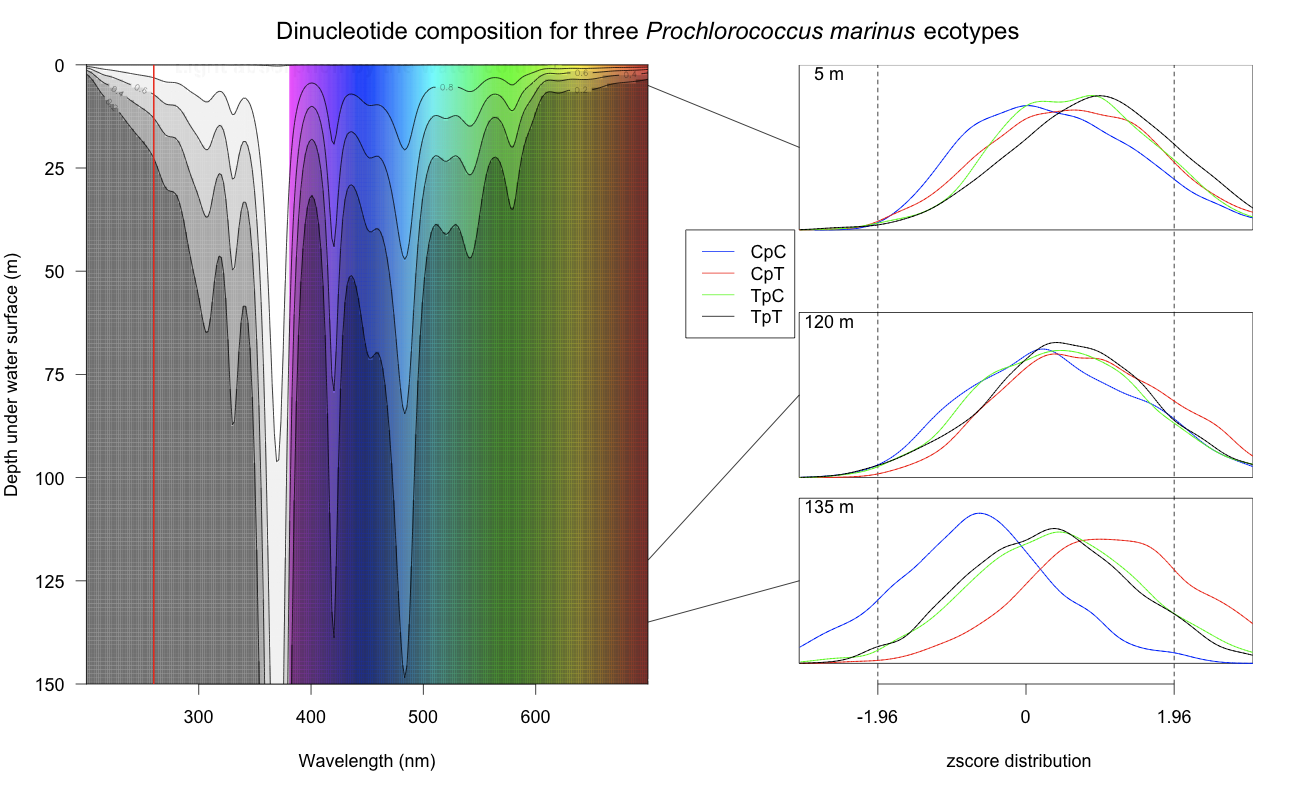
\includegraphics[width=\textwidth]{../figs/prochlo}
   \caption{This figure is from figure 2.7 in \cite{PalmeiraL2007},
    see also the example section in \texttt{data(prochlo)}. The left
    panel represents the absorbtion of light by pure water in the visible
    spectrum (gradient in color) and in the near UV (gradient in gray
    scale). Corresponding data were compiled from \cite{QuickendenTI1980}
    and \cite{LitjensRA1999}. For DNA, the biological relevant wavelength
    is at 260 nm (red vertical line) corresponding to its maximum for
    light absorbtion. The right panel shows the distribution of the
    $z$-codon statistic for the four pyrimidine dinucleotides (\textit{viz}
    CpC CpT TpC TpT) for the 
    coding sequences of three different ecotypes (5 m, 120 m, 135 m) of 
    \textit{Prochlorococcus marinus}. The complete genome sequences 
    accession numbers are BX548175 (\textit{P. marinus} MIT9313 
    \cite{RocapG2003} 5 m, high UV exposure), AE017126 (\textit{P. marinus}
    SS120 strain CCMP1375 \cite{DufresneA2003} 120 m, low UV exposure) 
    and BX548174 (\textit{P. marinus} MED4 \cite{RocapG2003} 135 m, 
    low UV exposure).
}
\label{fromdataprochlo}
\end{minipage}
}
\end{figure}


\section*{Session Informations}

This part was compiled under the following \Rlogo{}~environment:

\begin{itemize}
  \item R version 2.7.1 (2008-06-23), \verb|i386-apple-darwin8.8.2|
  \item Locale: \verb|fr_FR.UTF-8/fr_FR.UTF-8/fr_FR.UTF-8/C/C/C|
  \item Base packages: base, datasets, grDevices, graphics, methods,
    stats, utils
  \item Other packages: MASS~7.2-42, ade4~1.4-9, ape~2.2-1,
    nlme~3.1-89, quadprog~1.4-11, seqinr~1.1-7, tseries~0.10-15,
    xtable~1.5-2, zoo~1.5-4
  \item Loaded via a namespace (and not attached): grid~2.7.1,
    lattice~0.17-8, tools~2.7.1
\end{itemize}
There were two compilation steps:

\begin{itemize}
  \item \Rlogo{} compilation time was: Thu Jul 17 14:47:41 2008
  \item \LaTeX{} compilation time was: \today
\end{itemize}


% END - DO NOT REMOVE THIS LINE

%%%%%%%%%%%%  BIBLIOGRAPHY %%%%%%%%%%%%%%%%%
\clearpage
\addcontentsline{toc}{section}{References}
\bibliographystyle{plain}
\bibliography{../config/book}
\end{document}
